\graphicspath{{notes/6setsii/}}

\section{Set Theory, Part II}

In this chapter we return to set theory and consider several more-advanced constructions.

\subsection{Cartesian Products}

You have been working with Cartesian products for years, referring to a point in the plane $\R^2$ by its \emph{Cartesian coordinates} $(x,y)$. The basic idea is that each of the coordinates $x$ and $y$ is a member of the set $\R$. The same approach can be used for any two sets.

\begin{defn}
Let $A$ and $B$ be sets. The \textbf{Cartesian product} of $A$ and $B$ is the set
\[A\times B=\{(a,b):a\in A\text{ and }b\in B\}.\]
\end{defn}

\noindent $A\times B$ is simply the set of \emph{ordered pairs} $(a,b)$ where $a\in A$ and $b\in B$. Two ordered pairs $(a,b)$ and $(c,d)$ are equal if and only if their coordinates agree: $a = c$ and $b = d$.

\begin{examples}
	\item The Cartesian product of the real line $\R$ with itself is the $xy$-plane: rather than writing $\R\times\R$ which is unwieldy, we write $\R^2$.
	\[\R^2=\R\times\R=\{(x,y):x,y\in\R\}.\]
	More generally, $\R^n=\underbrace{\R\times\R\times\cdots\R}_{\text{$n$ times}}$ is the set of $n$-tuples of real numbers:
	\[\R^n=\{(x_1,x_2,\ldots,x_n):x_1,x_2,\ldots,x_n\in\R\}.\]
	\item If $A=\{1,2,3\}$ and $B=\{\alpha,\beta\}$, then the Cartesian product of $A$ and $B$ is
	\[A\times B=\{(1,\alpha),\ (1,\beta),\ (2,\alpha),\ (2,\beta),\ (3,\alpha),\ (3,\beta)\}\]
	Notice that this is a \emph{different set} to the Cartesian product of $B$ and $A$:
	\[B\times A=\{(\alpha,1),\ (\beta,1),\ (\alpha,2),\ (\beta,2),\ (\alpha,3),\ (\beta,3)\}\]
	\item Suppose you go to a restaurant where you have a choice of one main course and one side. The menu might be summarized set-theoretically: consider the sets
	\begin{gather*}
	\text{Mains}=\{\text{fish, steak, eggplant, pasta}\}\\
	\text{Sides}=\{\text{asparagus, salad, potatoes}\}
	\end{gather*}
	The Cartesian product Mains\,$\times$\,Sides is the set of all possible meals made up of one main and one side. It should be obvious that there are $4\times 3=12$ possible meal choices.
\end{examples}

% \begin{example}
% Let $f : A \to B$ be a function. The \emph{graph} of $f$ is the following subset of the Cartesian product $A \times B$:
% \[
% \Gamma(f) = \{(a, f(a)) : a \in A\} \subseteq A \times B.
% \]

% So, for example, the graph of the function $f(x) = x^2$ from $\R$ to $\R$ is a subset of the plane $\R \times \R = \R^2$ consisting of ordered pairs $(x, f(x)) = (x, x^2)$ for $x \in \R$. If you plot these ordered pairs, you will end up drawing the parabola that you expect.
% \end{example}

\noindent These last two examples illustrates the next theorem, which explains the use of the word \emph{product.}

\begin{thm}
If $A$ and $B$ are finite sets, then $\nm{A\times B}=\nm A\cdot\nm B$.
\end{thm}

\begin{proof}
Label the elements of each set and list the elements of $A\times B$ lexicographically. If $\nm A=m$ and $\nm B=n$, then we have:
\[\begin{array}{rccccccl}
A\times B=\big\{&(a_1,b_1),&(a_1,b_2),&(a_1,b_3),&\cdots&(a_1,b_n),&\\
&(a_2,b_1),&(a_2,b_2),&(a_2,b_3),&\cdots&(a_2,b_n),&\\
&\vdots&\vdots&\vdots&&\vdots&\\
&(a_m,b_1),&(a_m,b_2),&(a_m,b_3),&\cdots&(a_m,b_n)&\big\}
\end{array}\]
It should be clear that every element of $A\times B$ is listed exactly once. There are $m$ rows and $n$ columns, thus $\nm{A\times B}=mn$.
\end{proof}

Before we go any further, consider the complement of a Cartesian product $A\times B$. If you had to guess an expression for $\comp{(A\times B)}$, you might well try $\comp A\times\comp B$. Let us think more carefully.
% \begin{align*}
% (x,y)\in\comp{(A\times B)}&\iff (x,y)\not\in A\times B&&(x,y)\in\comp A\times\comp B\iff x\not\in A\text{ and }x\not\in B\\
% &\iff \neg((x,y)\in A\times B)&&\\
% &\iff \neg(x\in A\text{ and }y\in B)&&\\
% &\iff x\not\in A\text{ or }y\not\in B&&
% \end{align*}
\begin{gather*}
\begin{aligned}
(x,y)\in\comp{(A\times B)}&\iff (x,y)\not\in A\times B\\
&\iff \neg((x,y)\in A\times B)\\
&\iff \neg(x\in A\text{ and }y\in B)\\
&\iff x\not\in A\text{ or }y\not\in B
\end{aligned}
\end{gather*}
However $(x,y)\in\comp A\times\comp B\iff x\not\in A\text{ and }x\not\in B$. Since the definition of Cartesian product involves \emph{and,} its negation, by De Morgan's laws, involves \emph{or.} It follows that the complement of a Cartesian product is \emph{not a Cartesian product!} For more on this, see Exercise \hyperref[ex:cartneg]{\thesubsection.\ref*{ex:cartneg}}.\\


As an example of a basic set relationship involving Cartesian products, we prove a theorem.

\begin{thm}\label{thm:cartex}
Let $A,B,C,D$ be any sets. Then $(A\times B)\cup(C\times D)\subseteq(A\cup C)\times(B\cup D)$.
\end{thm}

\begin{proof}
Since we are dealing with Cartesian products, the general element has the form $(x,y)$.\\
\noindent\begin{minipage}{0.65\textwidth}
Let $(x,y)\in(A\times B)\cup(C\times D)$. Then 
\[(x,y)\in A\times B\qquad \text{or}\qquad (x,y)\in C\times D.\]
But then
\[(x\in A\text{ and }y\in B)\qquad\text{or}\qquad(x\in C\text{ and }y\in D).\]
Clearly $x\in A$ or $x\in C$, so $x\in A\cup C$.\\
Similarly $y\in B$ or $y\in D$, so $y\in B\cup D$.\\
Therefore $(x,y)\in (A\cup C)\times(B\cup D)$, as required.
\end{minipage}
\qquad
\begin{minipage}{0.28\textwidth}
\centering
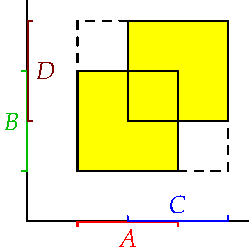
\includegraphics[width=\textwidth]{setsii-04-cartesian}
\end{minipage}
\end{proof}

\noindent The picture is an visualization of the theorem, where we assume that the sets $A,B,C$ and $D$ are all intervals of real numbers. $(A\times B)\cup(C\times D)$ is the yellow shaded region, while $(A\cup C)\times(B\cup D)$ is the larger dashed square. While helpful, the picture is not a proof! The theorem is a statement about \emph{any} sets, whereas the picture implicitly assumes that these sets are intervals.\\
For an application of the picture, it should be clear that if $x\in C\setminus A$ and $y\in B\setminus D$, then $(x,y)\in (A\cup C)\times (B\cup D)$ but $(x,y)\not\in (A\times B)\cup(C\times D)$. We do not therefore expect these sets to be equal.

% \paragraph{Self-test Questions}

% 	\begin{enumerate}
%     \item The Cartesian product of sets $A$ and $B$ is \underline{\phantom{the set of ordered pairs $\{(a,b):a\in A,\ b\in B\}$,\qquad}}
%     \item True or false: $A\times B=\emptyset\iff A=B=\emptyset$.
%     \item True or false: The cardinality of $A\times B$ is at least as large as $\max(\nm A,\nm B)$.
%   \end{enumerate}

\subsection*{Reading Questions}

\begin{enumerate}
    \item Let $A$ and $B$ be sets. Let $(a,b), (c,d) \in A \times B$. Then $(a,b) = (c,d)$ if and only if 
    \begin{enumerate}
        \item $a = c$
        \item $b = d$
        \item $ad = bc$
        \item $a = c$ and $b = d$
    \end{enumerate}
    
    \item True or False: $A \times B = \emptyset$ if and only if $A = B = \emptyset$.
    
    \item Fill in the blank: If $A$ and $B$ are both finite nonempty sets, then $\max(|A|, |B|) \quad \rule{0.75cm}{0.15mm} \quad |A \times B|$.
    \begin{enumerate}
        \item $=$
        \item $\geq$
        \item $\leq$
        \item $\neq$
    \end{enumerate}
\end{enumerate}

\subsection*{Practice Problems}

\begin{enumerate}\renewcommand{\labelenumi}{\thesubsection.\theenumi}
\item Let $A,B,C,D$ be sets. Prove
\[
(A \times B) \cap (C \times D) = (A \cap C) \times (B \cap D).
\]

\href{https://youtu.be/TpjjI0dCfok}{Video Solution}

\item Let $A$ and $B$ be nonempty sets. Define a function $\pi_1 : A \times B \to A$ by $\pi_1(a,b) = a$. Show $\pi_1$ is surjective. Under what conditions is it a bijection?

\href{https://youtu.be/qIhugCqylC0}{Video Solution}
\end{enumerate}

\subsection*{Exercises}

\begin{enumerate}\renewcommand{\labelenumi}{\thesubsection.\theenumi}
  \item\begin{enumerate}
    \item Suppose that $A=\{1,2\}$ and $B=\{3,4,5\}$. State the sets $A\times B$ and $B\times \emptyset$ in roster notation.
    \item Sketch both $A\times B$ and $B\times A$ using dots on the plane. What do you observe about your pictures?
    \item If $A,B,C$ are any sets, we may define the triple Cartesian product as
    \[A\times B\times C=\big\{(a,b,c):a\in A,\ b\in B,\ c\in C\big\}\]
    If $C=\{6,7\}$ and $A,B$ are as above, state the set $A\times B\times C$ in roster notation.
    \item For the sets $A$, $B$ and $C$ as above, is $A \times (B \times C) = A \times B \times C$? 
  \end{enumerate}
  
  \item Consider the following subintervals of the real line: $A=[2,5],\ B=(0,4)$.
  \begin{enumerate}
    \item Express the set $\comp{(A\setminus B)}$ in interval notation, as a disjoint union of intervals.
     \item Sketch the sets $A\times B$ and $\comp{(A \times B)}$ on the plane $\R^2$. (Submit two different drawings, one for the set $A \times B$ and one for its complement.)
    \item Sketch the set $\comp{(A\setminus B)}\times (B\setminus A)$ on the plane $\R^2$.
  \end{enumerate}

	\item Rewrite the condition
	\[(x,y)\in (\comp{A}\cup B)\times (C\setminus D)\]
	in terms of (some of) the following propositions:
	\[x\in A,\quad x\not\in A,\quad x\in B,\quad x\not\in B,\quad y\in C,\quad y\not\in C,\quad y\in D,\quad y\not\in D.\]

	\item Let $A=[1,3]$, $B=[2,4]$ and $C=[2,3]$. \emph{Prove or disprove} that
	\[(A\times B)\cap (B\times A)=C\times C.\]
	\emph{Hint: Draw the sets $A\times B$, $B\times A$ and $C\times C$ in the Cartesian plane. The picture will give you a hint on whether or not the statement is true, but it does not constitute a proof.}
	
	\item A straight line subset of the plane $\R^2$ is a subset of the form
	  \[A_{a,b,c}=\{(x,y):ax+by=c\},\quad\text{for some constants $a,b,c$, with $ab\neq 0$.}\]
	  \begin{enumerate}
	  \item Draw the set $A_{1,2,3}$. Is it a Cartesian product?
	 	\item Which straight line subsets in the plane $\R^2$ are Cartesian products? Otherwise said, find a condition on the constants $a,b,c$ for which the set $A_{a,b,c}$ is a Cartesian product.
		\end{enumerate}
	
	\item\label{ex:cartneg} Draw a picture, similar to that in Theorem \ref{thm:cartex}, which illustrates the fact that
	\[\comp{(A\times B)}\neq \comp A\times \comp B.\]
	Using your picture, write the set $\comp{(A\times B)}$ in the form
	\[(C_1\times D_1)\cup (C_2\times D_2)\cup\cdots\]
	where each of the unions are \emph{disjoint:} that is $i\neq j\implies (C_i\times D_i)\cap (C_j\times D_j)=\emptyset$. You don't have to prove your assertion.
		
	\item Prove that $A\cap B=\emptyset\iff (A\times B)\cap(B\times A)=\emptyset$.
	
	\item Let $A,B,C$ be sets. Prove
\begin{enumerate}
    \item $A \times (B \cup C) = (A \times B) \cup (A \times C)$.
    \item $A \times (B \cap C) = (A \times B) \cap (A \times C)$.
    \item $A \times (B \setminus C) = (A \times B) \setminus (A \times C)$.
\end{enumerate}

\item \begin{enumerate}
    \item Give an explicit example of sets $A,B,C,D$ such that $(A \times B) \cup (C \times D) \neq (A \cup C) \times (B \cup D)$.
    \item For sets $A,B,C,D$, prove that
    \[
        (A \cup C) \times (B \cup D) = (A \times B) \cup (A \times D) \cup (C \times B) \cup (C \times D).
    \]
\end{enumerate}

\item Let $A$ and $B$ be sets. Prove
\[
    \comp{(A \times B)} = (\comp{A} \times \comp{B}) \cup (\comp{A} \times B) \cup (A \times \comp{B}).
\]
	
  \item\begin{enumerate}
		\item Suppose that $\nm A=3$, and $\nm B=4$. What are the minimum and maximum values for the cardinalities $\nm{(A\times B)\cap(B\times A)}$ and $\nm{(A\times B)\cup(B\times A)}$?
		\item More generally, suppose that $\nm A=m$, $\nm B=n$ and $\nm{A\cap B}=c$. What are the above cardinalities?
	\end{enumerate}
	
  \item Prove the following by induction. For all $n\in\N$, if $A_1,\ldots,A_n$ are finite sets, then
  \[\nm{A_1\times\cdots\times A_n}=\nm{A_1}\cdots\nm{A_n}\] 
	
	\item Let $E\subseteq\N\times\N$ be the smallest subset which satisfies the following conditions:
	\begin{itemize}
		\item Base case: $(1,1)\in E$
		\item Generating Rule I: If $(a,b)\in E$ then $(a,a+b)\in E$
		\item Generating Rule II: If $(a,b)\in E$ then $(b,a)\in E$
	\end{itemize}

	\begin{enumerate}
		\item Show in detail that $(4,3)\in E$.
		\item Show by induction that for every $n\in\N$, $(1,n)\in E$.
		\item (Very hard!!!) Show that $E=\{(a,b)\in\N\times\N:\gcd(a,b)=1\}$. \emph{Think carefully about how the Euclidean algorithm works, and what the generating rules might have to do with it\ldots}
	\end{enumerate}
	
	\item A strict set-theoretic definition requires you to build the ordered pair $(a,b)$ as a set: typically $(a,b)=\{a,\{a,b\}\}$. One then proves that $(a,b)=(c,d)\iff a=c$ and $b=d$.
	\begin{enumerate}
	  \item One of the axioms of set theory (\emph{regularity}) says that there is no set $a$ for which $a\in a$. Use this to prove that the cardinality of $(a,b)=\{a,\{a,b\}\}$ is two.
	  \item Prove that $(a,b)=(c,d)\implies\begin{cases}
	  a=c\text{ and }b=d,\\
	  \qquad\quad\text{\emph{or}}\\
	  a=\{c,d\}\text{ and }c=\{a,b\}.
	  \end{cases}$
	  \item In the second case, prove that there exists a set $S$ such that $a\in S\in a$. The axiom of regularity also says that this is illegal. Conclude that $(a,b)=(c,d)\iff a=c$ and $b=d$.
	\end{enumerate}
	
	\item Let $A$ and $B$ be nonempty sets. Define functions $\pi_1 : A \times B \to A$ and $\pi_2 : A \times B \to B$ by $\pi_1(a,b) = a$ and $\pi_2(a,b) = b$ respectively (these are called the \emph{projection maps}). 
\begin{enumerate}
    \item If $A = B = \R$ and $X = [1,3]$, $Y = (2,4]$, then $X \times Y \subseteq A \times B$. Compute the images $\pi_1(X \times Y)$ and $\pi_2(X \times Y)$.
    \item Let $Z$ be any set and suppose there are functions $\rho_1 : Z \to A$ and $\rho_2 : Z \to B$. Show there is a unique function $h : Z \to A \times B$ such that $\rho_1 = \pi_1 \circ h$ and $\rho_2 = \pi_2 \circ h$.
\end{enumerate}
\end{enumerate}
\newpage

\subsection{Power Sets}

Thusfar we have seen how to build new sets from old using the operations of subset, complement, union, intersection and Cartesian product. There is essentially only one further method whereby we can produce new sets; given a set $A$, we consider the collection of all of the subsets of $A$ and we insist that this collection is a set.

\begin{defn}
The \textbf{power set} of $A$ is the set $\cP(A)$ of all subsets of $A$. That is,
\[\cP(A)=\{B:B\subseteq A\}.\]
Otherwise said: $B\in\cP(A)\iff B\subseteq A$.
\end{defn}

\begin{examples}
	\item Let $A=\{1,3,7\}$. Then $A$ has the following subsets, listed by how many elements are in each subset.
\[\begin{array}{ll}
\text{0-elements:}&\emptyset\\
\text{1-element:}&\{1\},\ \{3\},\ \{7\}\\
\text{2-elements:}&\{1,3\},\ \{1,7\},\ \{3,7\}\\
\text{3-elements:}&\{1,3,7\}
\end{array}\]
Gathering these together, we have the power set:
\[\cP(A)=\Bigl\{\emptyset,\{1\},\{3\},\{7\},\{1,3\},\{1,7\},\{3,7\},\{1,3,7\}\Bigr\}.\]
\item Consider $B=\Bigl\{1,\bigl\{\{2\},3\bigr\}\Bigr\}$. It is essential that you use different size set brackets to prevent confusion. $B$ has only \emph{two} elements, namely $1$ and $\bigl\{\{2\},3\bigr\}$. We can gather the subsets of $B$ in a table.
\[\begin{array}{ll}
\text{0-elements:}&\emptyset\\
\text{1-element:}&\{1\},\ \Bigl\{\bigl\{\{2\},3\bigr\}\Bigr\}\\
\text{2-elements:}&\Bigl\{1,\bigl\{\{2\},3\bigr\}\Bigr\}
\end{array}\]
In the second line, remember that to make a subset out of a single element you must surround the element with set brackets. Thus $1\in B\implies \{1\}\subseteq B$ and
\[\bigl\{\{2\},3\bigr\}\in B\implies \Bigl\{\bigl\{\{2\},3\bigr\}\Bigr\}\subseteq B.\]
The power set of $B$ is therefore
\[\cP(B)=\biggl\{\emptyset,\ \{1\},\ \Bigl\{\bigl\{\{2\},3\bigr\}\Bigr\},\ \Bigl\{1,\bigl\{\{2\},3\bigr\}\Bigr\}\biggr\}.\]
\end{examples}\pagebreak[2]


\paragraph{Notation}

Be absolutely certain that you understand the difference between $\in$ and $\subseteq$. It is easy to become confused when considering power sets. In the context of the previous examples, here are eight propositions. Which are true and which are false?\footnote{Only (a), (d), and (g) are true. Make sure you understand why!}
\[\begin{array}{r@{\quad}l@{\qquad\qquad}r@{\quad}l@{\qquad\qquad}r@{\quad}l@{\qquad\qquad}r@{\quad}l}
\text{(a)}&1\in A
		&\text{(b)}&1\in\cP(A)
		&\text{(c)}&\{1\}\in A
		&\text{(d)}&\{1\}\in\cP(A)\\
\text{(e)}&1\subseteq A
		&\text{(f)}&1\subseteq\cP(A)
		&\text{(g)}&\{1\}\subseteq A
		&\text{(h)}&\{1\}\subseteq\cP(A)
\end{array}\]

\noindent As a further exercise in being careful with notation, consider the following theorem.

\begin{thm}\label{thm:powersub}
If $A\subseteq B$, then $\cP(A)\subseteq\cP(B)$.
\end{thm}

\begin{proof}
Suppose that $A\subseteq B$ and let $C\in\cP(A)$. We must show that $C\in\cP(B)$.\\
By definition, $C\in\cP(A)\implies C\subseteq A$. Since subset inclusion is transitive (Theorem \hyperlink{thm:subsettranslnk}{\ref*{thm:subsettrans}}), we have
\[C\subseteq A\subseteq B\implies C\subseteq B.\]
This says that $C\in\cP(B)$. Therefore $\cP(A)\subseteq\cP(B)$.
\end{proof}

\noindent It is very easy to get confused by the proof of this theorem. Exercises \hyperref[ex:powersub1]{\thesubsection.\ref*{ex:powersub1}} and \hyperref[ex:powersub2]{\thesubsection.\ref*{ex:powersub2}} discuss things further.


\subsubsection*{Cardinality and Power Sets}

Let's investigate how the cardinality of a set and its power set are related. Consider a few basic examples where we list all of the subsets, grouped by cardinality.
\[\begin{array}{|c||c|c|c|c||c|}
\hline
\text{Set }A&\text{0-elements}&\text{1-element}&\text{2-elements}&\text{3-elements}&\nm{\cP(A)}\\\hline
\emptyset&\emptyset&&&&1\\\hline
\{a\}&\emptyset&\{a\}&&&1+1=2\\\hline
\{a,b\}&\emptyset&\{a\},\{b\}&\{a,b\}&&1+2+1=4\\\hline
\{a,b,c\}&\emptyset&\{a\},\{b\},\{c\}&\{a,b\},\{a,c\},\{b,c\}&\{a,b,c\}&1+3+3+1=8\\\hline
\end{array}\]
You should have seen this pattern before: we are looking at the first few lines of Pascal's Triangle.\footnote{If you know a little about combinations from probability, it should be clear that a set $A$ with $n$ elements has precisely ${}^nC_r=\binom nr=\frac{n!}{r!(n-r)!}$ distinct $r$-element subsets.} It should be no surprise that if $\nm A=4$, then $\nm{\cP(A)}=1+4+6+4+1=16$. The progression $1,2,4,8,16,\ldots$ in the final column immediately suggests the following theorem.

\begin{thm}\label{thm:powercard}
Suppose that $A$ is a finite set. Then $\nm{\cP(A)}=2^{\nm A}$.
\end{thm}

\noindent Conjuring up a proof may seem daunting given how little we know about $A$! In fact we have only one thing to work with: the \emph{cardinality} of $A$. Indeed you might find it helpful to rephrase the theorem as follows:
\[\forall n\in\N_0,\ \ \nm A=n\implies \nm{\cP(A)}=2^{n}\]
Viewed this way, we see that we want to prove an infinite collection of propositions, indexed by the set $\N_0$:  induction seems like the way forward. What might the induction step look like? The basic idea is that every set with $n+1$ elements is the disjoint union of a set with $n$ elements and a single-element set. The induction step is essentially the observation that any $n+1$-element set $B$ has \emph{twice} the number of subsets of some $n$-element set $A$. It is instructive to see an example of this before writing the proof. 

\begin{example}
Let $B=\{1,2,3\}$. Now choose the element $3\in B$ and delete it to create the smaller set
\[A=\{1,2\}=B\setminus\{3\}.\]
We can split the subsets of $B$ into two groups: those which contain 3 and those which do not. In the following table we list all of the subsets of $B$. In the first column are those subsets $X$ which do not contain 3. These are exactly the subsets of $A$. In the second column are the subsets $Y=X\cup\{3\}$ of $B$ which do contain 3.
\[\begin{array}{c|c}
X&X\cup\{3\}\\\hline
\emptyset&\{3\}\\
\{1\}&\{1,3\}\\
\{2\}&\{2,3\}\\
\{1,2\}&\{1,2,3\}
\end{array}\]
It is clear that $B$ has twice the number of subsets of $A$.
\end{example}

\noindent This method of pairing is exactly mirrored in the proof.

\begin{proof}
We prove by induction on the cardinality of $A$. For each $n\in\N_0$, we consider the proposition
\[\nm A=n\implies\nm{\cP(A)}=2^n.\tag*{($\ast$)}\]
(\emph{Base Case})\quad If $n=0$, then $A=\emptyset$ (Theorem \hyperlink{thm:subsettranslnk}{\ref*{thm:subsettrans}}). But then $\cP(A)=\{\emptyset\}$, whence $\nm{\cP(A)}=1=2^0$.\\
(\emph{Induction Step})\quad Fix $n\in\N_0$ and assume that ($\ast$) is true for this $n$. That is, we assume that any set with $n$ elements has $2^n$ subsets. Now let $B$ be \emph{any} set with $n+1$ elements. Choose one of the elements $b\in B$ and define $A=B\setminus\{b\}$. The subsets of $B$ can then be separated into the following two types:
\begin{enumerate}\itemsep0pt
  \item Subsets $X\subseteq B$ which do not contain $b$.
  \item Subsets $Y\subseteq B$ which contain $b$.
\end{enumerate}
In the first case, $X$ is really a subset of $A$.\\
In the second case we can write $Y=X\cup\{b\}$, where $X$ is again a subset of $A$.\\
Each subset $X\subseteq A$ therefore corresponds to precisely two subsets $X$ and $X\cup\{b\}$ of $B$. Since $\nm{A}=n$, the induction hypothesis tells us that there are $2^n$ subsets $X\subseteq A$, whence
\[\nm{\cP(B)}=2\nm{\cP(A)}=2^{n+1}.\]
By induction, $(\ast)$ is true for all $n\in\N_0$.
\end{proof}

\noindent Once you understand the proof, you should compare it to the proof of Theorem \ref{thm:polygon} on the interior angles of a polygon: the idea is very similar. Exercise \hyperref[ex:binom]{\thesubsection.\ref*{ex:binom}} gives an alternative proof of this result.\\

\noindent As a final example, we consider the interaction of power sets and Cartesian products.

\begin{example}
Suppose that $A=\{a\}$ and $B=\{b,c\}$. Then
\[A\times B=\{(a,b),(a,c)\}.\]
The power set $\cP(A\times B)$ therefore contains $2^2=4$ elements: indeed
\[\cP(A\times B)=\Big\{\emptyset,\ \{(a,b)\},\ \{(a,c)\},\ \{(a,b),(a,c)\}\Big\}.\]
The power sets of $A$ and $B$ have 2 and 4 elements respectively:
\[\cP(A)=\big\{\emptyset,\{a\}\big\},\qquad\cP(B)=\big\{\emptyset,\{b\},\{c\},\{b,c\}\big\}.\]
The Cartesian product of the power sets therefore has $2\times 4=8$ elements:
\begin{multline*}
\cP(A)\times\cP(B)
=\Big\{\big(\emptyset,\emptyset\big),\  \big(\emptyset,\{b\}\big),\  \big(\emptyset,\{c\}\big),\  \big(\emptyset,\{b,c\}\big),\\*
\big(\{a\},\emptyset\big),\  \big(\{a\},\{b\}\big),\  \big(\{a\},\{c\}\big),\  \big(\{a\},\{b,c\}\big)\Big\}.
\end{multline*}
It should be clear from this example not only that $\cP(A\times B)\neq\cP(A)\times\cP(B)$, but that the elements of the two sets are completely different. The elements of $\cP(A\times B)$ are \emph{sets of ordered pairs,} while the elements of $\cP(A)\times\cP(B)$ are \emph{ordered pairs of sets.}
\end{example}



% \paragraph{Self-test Questions}

% 	\begin{enumerate}
%     \item The power set of a set $A$ is \underline{\phantom{the set of all subsets of $A$\qquad\qquad\qquad}}
%     \item Which of the following are correct statements?
%     \[[0,1)\in\cP(\R),\qquad 7\in\cP(\N),\qquad \{(3,5),(2,9)\}\subseteq\cP(\N\times\N),\qquad \{4,\pi\}\in\cP(\R)\]
%   \end{enumerate}

\subsection*{Reading Questions}

\begin{enumerate}
    \item Which of the following are true statements. Select all that apply.
    \begin{enumerate}
        \item $[0,1) \in \cP(\R)$
        \item $7 \in \cP(\N)$
        \item $\{(3,5),(2,9)\} \subseteq \cP(\N \times \N)$
        \item $\{4, \pi\} \in \cP(\R)$
    \end{enumerate}
    
    \item Let $A = \{(1,2), 3, (4,\{5\})\}$. What is $|\cP(A)|$?
    \begin{enumerate}
        \item $3$
        \item $8$
        \item $16$
        \item $32$
    \end{enumerate}
\end{enumerate}

\subsection*{Practice Problems}

\begin{enumerate}\renewcommand{\labelenumi}{\thesubsection.\theenumi}
\item Let $A = \{\emptyset, 1, \{a\}\}$. List the elements of $\cP(A)$, compute its cardinality. Then answer True or False for the following:
\begin{enumerate}
    \item $\emptyset \in A$
    \item $\emptyset \subseteq A$
    \item $\emptyset \in \cP(A)$
    \item $\emptyset \subseteq \cP(A)$
    \item $\{\{a\}\} \subseteq \cP(A)$
    \item $\{\{\emptyset, 1\}, \{\emptyset\}, \emptyset\} \subseteq \cP(A)$
    \item $A \in \cP(A)$
    \item $A \subseteq \cP(A)$
\end{enumerate}

\href{https://youtu.be/Pprf24H6SLc}{Video Solution}

\item Prove that $A \subseteq B$ if and only if $\cP(A) \subseteq \cP(B)$. 

\href{https://youtu.be/24tLpM3qdMM}{Video Solution}
\end{enumerate}


\subsection*{Exercises}

\begin{enumerate}\renewcommand{\labelenumi}{\thesubsection.\theenumi}
  \item Write the following sets in roster notation:\\[5pt]
	\begin{tabular}{r@{\ \ }l@{\qquad\qquad\qquad\qquad}r@{\ \ }l}
	(a)& $\cP(A)$ \text{for } $A=\{1,2\}$.&(d)& $\cP(A)$ \text{for } $A=\{\emptyset,3,\{4\}\}$.\\[2pt]
	(b)&$\cP(A)$ \text{for } $A=\{1,2,3\}$.&(e)& $\cP(\cP(A))$ \text{for } $A=\{3,5\}$.\\[5pt]
	(c)&$\cP(A)$ \text{for } $A=\bigl\{(1,2),(2,3)\bigr\}$.&(f)& $\{ X \in \cP(\{1,2,3,4\}) \colon |X| = 1 \}$.
	\end{tabular}
	
	\item Let $A=\{1,3\}$ and $B=\{2,4\}$.
	\begin{enumerate}
	  \item Draw a picture of the set $A\times B$.
	  \item Compute $\cP(A\times B)$.
	  \item What is the cardinality of $\cP(A)\times\cP(B)$? \emph{Don't compute the set!}
	\end{enumerate}
  
	\item Determine whether the following statements are true or false (\emph{in (b), the symbol $\subsetneq$ means `proper subset'}). Justify your answers.
  \begin{enumerate}
    \item If $\{7\}\in\cP(A)$, then $7\in A$ and $\{7\}\notin A$.
    \item Suppose that $A,B$ and $C$ are sets such that $A\subsetneq\cP(B)\subsetneq C$ and $\nm A=2$. Then $\nm C$ can be 5, but $\nm C$ cannot be 4.
    \item If a set $B$ has one more element than a set $A$, then $\cP(B)$ has at least two more elements than $\cP(A)$.
    \item Suppose that the sets $A,B,C$ and $D$ are all subsets of $\{1,2,3\}$ with cardinality two. Then at least two of these sets are equal. 
  \end{enumerate}
  
	\item\label{ex:powersub1} Here are three incorrect proofs of Theorem \ref{thm:powersub}. Explain why each fails.
	\begin{enumerate}
		\item Let $x\in\cP(A)$. Then $x\in A$. Since $A\subseteq B$, we have $x\in B$. Therefore $x\in\cP(B)$, and so $\cP(A)\subseteq\cP(B)$.
		\item Let $A=\{1,2\}$ and $B=\{1,2,3\}$. Then $\cP(A)=\{\emptyset,\{1\},\{2\},A\}$, and\\
		$\cP(B)=\{\emptyset,\{1\},\{2\},\{3\},\{1,2\},\{1,3\},\{2,3\},B\}$. Thus $\cP(A)\subseteq\cP(B)$.
		\item Let $x\in A$. Since $A\subseteq B$, we have $x\in B$. Since $x\in A$ and $x\in B$, we have $\{x\}\in\cP(A)$, and $\{x\}\in\cP(B)$.
	\end{enumerate}
	
	\item\label{ex:powersub2} Consider the converse of Theorem \ref{thm:powersub}. Is it true or false? Prove or disprove your conjecture.
	
	\item\begin{enumerate}
	  \item Prove that $\cP(A)\cup\cP(B)\subseteq\cP(A\cup B)$. Provide a counter-example to show that we do not expect equality.
	  \item Does anything change if you replace $\cup$ with $\cap$ in part (a)? Justify your answer.
	\end{enumerate}

 \item Let $A$ and $B$ be sets. Prove or disprove: $A \subseteq B \implies \cP(A) \subseteq \cP(B)$.

 
	\item \begin{enumerate} \item For any set $A$, show there is an injection $\iota : A \to \cP(A)$. (Explicitly construct a map, and show that it is one-to-one.)
\item Is there any set $A$ such that $A \cap \cP(A) \neq \emptyset$?
\end{enumerate}

\item If we define an ordered pair $(a,b)$ as $\{\{a\}, \{a,b\}\}$, show that $A \times B \subseteq \cP(\cP(A \cup B))$.
	
	\item Consider the proof of Theorem \ref{thm:powercard}. Let $B$ be a set with $n+1$ elements, let $b\in B$ and let $A=B\setminus\{b\}$. Prove that the function $f:\cP(A)\times\{1,2\}\to\cP(B)$ defined by
	\[f(X,1)=X,\qquad f(X,2)=X\cup\{b\}\]
	is a bijection, and that consequently, by Theorem \ref{thm:finitecard}, $\nm{\cP(A)\times\{1,2\}}=\nm{\cP(B)}$.
	
	\item\label{ex:binom} We use the following notation for the binomial coefficient: $\binom nr=\frac{n!}{r!(n-r)!}$. This symbol denotes the number of distinct ways one can choose $r$ objects from a set of $n$ objects.
	\begin{enumerate}
	  \item Use the definition of the binomial coefficient to prove the following:
	  \[\text{If } 1\le r\le n,\ \text{ then }\ \binom{n+1}r=\binom nr+\binom n{r-1}.\]
		\item Prove by induction that $\forall n\in\N_0,\,\sum\limits_{r=0}^n\binom nr=2^n$.\\
		\emph{Hint: Use part (a) in the induction step. Note that the smallest $n$ for which it applies is $n=1\ldots$}
		\item Explain why part (b) provides an alternative proof of Theorem \ref{thm:powercard}.
	\end{enumerate}
	\emph{If you found this easy, try proving the binomial theorem: $\forall n\in\N,\,(x+y)^n=\sum\limits_{r=0}^n\binom nrx^ry^{n-r}$.}
	
	\item Let $A$ and $B$ be nonempty sets. We use the notation $A^B$ to denote the set of all functions from $B$ to $A$. 
\begin{enumerate}
    \item If $A = \{0,1\}$ and $B = \{a,b,c\}$, list all elements of $A^B$. What is $|A^B|$?
    \item If $A$ and $B$ are finite sets, show $|A^B| = |A|^{|B|}$.
    \item Let $B$ be a set and $Y \subseteq B$. Define $\chi_Y : B \to \{0,1\}$ by
    \[
        \chi_Y(x) = \begin{cases}
        1 & \text{ if } x \in Y \\
        0 & \text{ if } x \notin Y.
        \end{cases}
    \]
    We call $\chi_Y$ the \emph{characteristic function} of $Y$. By definition, $\chi_Y \in \{0,1\}^B$ for any $Y \subseteq B$. Show every element of $\{0,1\}^B$ is the characteristic function of some subset of $B$. In other words, prove that for all $f \in \{0,1\}^B$, there exists $Y \subseteq B$ such that $f = \chi_Y$.
    \item Let $B$ be a set. Define $\Phi : \cP(B) \to \{0,1\}^B$ by $\Phi(Y) = \chi_Y$. Show that $\Phi$ is a bijection.
    \item If $B$ is finite, conclude that $|\cP(B)| = |\{0,1\}^B| = 2^{|B|}$.
\end{enumerate}

\item Let $A,B,C,D$ be nonempty sets. Suppose that there is a bijection $f : A \to B$ and a bijection $g : C \to D$. Show there is a bijection between $C^A$ and $D^B$.

\item Let $X$ be an infinite set. A collection of sets $\mathcal{F} \subseteq \cP(X)$ is called a \emph{filter} if the following conditions are satisfied:
\begin{enumerate}[label=(\arabic*)]
    \item $\emptyset \notin \mathcal{F}$ and $X \in \mathcal{F}$,
    \item if $A \subseteq B \subseteq X$ and $A \in \mathcal{F}$, then $B \in \mathcal{F}$,
    \item if $A,B \in \mathcal{F}$, then $A \cap B \in \mathcal{F}$.
\end{enumerate}
Filters are meant to capture a notion of largeness for sets.
\begin{enumerate}
    \item Show that $\{A : X \setminus A \text{ is finite}\}$ is a filter (this is called the \emph{cofinite} or \emph{Frech\'et filter}).
    \item A filter $\mathcal{U} \subseteq \cP(X)$ is called an \emph{ultrafilter} if it is a filter and for any $A \in \cP(X)$, we have either $A \in \mathcal{U}$ or $X \setminus A \in \mathcal{U}$. Show that the cofinite filter is not an ultrafilter.
    \item Show that a filter $\mathcal{F}$ is an ultrafilter if and only if for any $A_1,\ldots,A_n \in \cP(X)$ such that $A_1 \cup \cdots \cup A_n \in \mathcal{F}$, there is $1 \leq i \leq n$ such that $A_i \in \mathcal{F}$.
    \item Let $s \in X$, and define $\mathcal{U}_s = \{A \in \cP(X) : s \in A\}$. Show $\mathcal{U}_s$ is an ultrafilter, called the \emph{principal ultrafilter generated by $s$}.
    \item An ultrafilter $\mathcal{U}$ is \emph{nonprincipal} if it is not equal to $\mathcal{U}_s$ for any $s \in X$. Show an ultrafilter $\mathcal{U}$ is nonprincipal if and only if it contains the cofinite filter (as a subset).
\end{enumerate}
\end{enumerate}
\newpage

\subsection{Indexed Collections of Sets}

In this section we consider collections of sets $A_n$, where each $n$ lies in some \emph{indexing set} $I$. It is often the case that $I=\N$ or $\Z$. If $I$ is some other set, for example the real numbers $\R$, the label for the index may be chosen accordingly: e.g. $A_x$.

% \begin{examples}
% 	\item Let $A_n=[-n,n]\subseteq \R$, for each $n\in\N$. For example $A_1=[-1,1]$, $A_2=[-2,2]$, etc.
% 	\item Let $A_n=(n,n+1]\subseteq\R$, for each $n\in\Z$. E.g.\ $A_{-17}=(-17,-16]$.
% 	\item Let $A_n=[0,\frac 1n)\subseteq\R$, for each $n\in\N$. E.g.\ $A_{1000}=[0,\frac 1{1000})$.
% 	\item Let $A_n=(0,\frac 1n)\subseteq\R$, for each $n\in\N$.
% 	\item Let $A_n=\{x\in\R:\nm{x^2-1}<\frac 1n\}$, for each $n\in\N$. Here $A_3=\Big(-\sqrt{\frac 43},-\sqrt{\frac 23}\Big)\cup \Big(\sqrt{\frac 23},\sqrt{\frac 43}\Big)$.
% \end{examples}

\begin{defn}\label{defn:indexed}
Given a family of indexed sets $\{A_n:n\in I\}$, we may form the \textbf{union} and \textbf{intersection} of the collection:
\begin{gather*}
\bigcup_{n\in I}A_n=\{x:x\in A_n\text{\emph{ for some} }n\in I\},\\
\bigcap_{n\in I}A_n=\{x:x\in A_n\text{\emph{ for all} }n\in I\}.
\end{gather*}
Otherwise said,
\begin{gather*}
x\in\bigcup_{n\in I}A_n\iff \exists n\in I\text{ such that }x\in A_n\\
x\in\bigcap_{n\in I}A_n\iff \forall n\in I\text{ we have }x\in A_n
\end{gather*}
A indexed collection $\{A_n:n\in I\}$ is \textbf{pairwise disjoint} if $A_m\cap A_n=\emptyset$ whenever $m\neq n$.
\end{defn}

\noindent When the indexing set is $\N$, it is common to use the notations $\bigcup\limits_{n=1}^\infty A_n$ and $\bigcap\limits_{n=1}^\infty A_n$.

\begin{example}
Let the indexing set be $I=\{\alpha,\beta,\gamma\}$, and let
\[A_\alpha=\{1,3,5\},\qquad A_\beta=\{2,3,4,6\},\qquad A_\gamma=\{1,2,3,6\}.\]
It should be clear that
\[\bigcup_{i\in I}A_i=A_\alpha\cup A_\beta\cup A_\gamma=\{1,2,3,4,5,6\}\]
and
\[\bigcap_{i\in I}A_i=A_\alpha\cap A_\beta\cap A_\gamma=\{3\}\]
\end{example}

\noindent The following Theorem is almost immediate given the definitions of union and intersection: can you supply a formal proof?

\begin{thm}
Let $\{A_n:n\in I\}$ be an indexed collection of sets, and let $m\in I$. Then
\[A_m\subseteq\bigcup_{n\in I}A_n\quad\text{and}\quad \bigcap_{n\in I}A_n\subseteq A_m.\]
\end{thm}



% \begin{proof}
% \begin{enumerate}
% 	\item Let $x\in A_m$. Then $\exists i\in I$ such that $x\in A_i$, and hence $x\in\bigcup\limits_{i\in I}A_i$.
% 	\item Let $x\in\bigcap\limits_{i\in I}A_i$. Then $\forall i\in I$ we have $x\in A_i$. In particular, $x\in A_j$.\qedhere
% \end{enumerate}
% \end{proof}


\subsubsection*{Infinite Unions and Intersections: don't take limits!}

The challenge with indexed sets often involves computing unions and intersections of \emph{infinitely many} sets. Be very careful with this: it is very tempting to `take limits' when this doesn't make sense. With this in mind, we dissect an important example.\\

\noindent For each $n\in\N$, consider the interval $A_n=\Bigl[0\,,\,\frac 1n\Bigr)$. We analyze the collection $\{A_n:n\in\N\}$. First observe that $m\le n\implies \frac 1n\le \frac 1m\implies A_n\subseteq A_m$; the sets are therefore \textbf{nested}:
\[A_1\supseteq A_2\supseteq A_3\supseteq A_4\supseteq\cdots\tag*{($\ast$)}\]
Since every set in the collection is a subset of $A_1$, it follows that this is the union,
\[\bigcup_{n=1}^\infty A_n=A_1=[0,1).\]
Before considering the full intersection, we first compute all finite intersections. Since the sets $A_n$ are nested in the form ($\ast$), it follows that any \emph{finite} intersection is simply the smallest of the listed sets: i.e., for any constant $m\in\N$ we have
\[\bigcap_{n=1}^mA_n=A_m=\Bigl[0\,,\,\frac 1m\Bigr).\]
Observe that this is non-empty \emph{for every $m$}. Now what about the infinite intersection? You might be tempted to take a limit and make an argument such as
\[\bigcap\limits_{n=1}^\infty A_n\overset{?}{=}\lim_{m\to\infty}\bigcap_{n=1}^mA_n\overset{?}{=}\lim_{m\to\infty}\Bigl[0\,,\,\frac 1m\Bigr)\overset{?}{=}\Bigl[0\,,\lim_{m\to\infty}\frac 1m\Bigr)=[0,0).\]
Quite apart from the issue that $[0,0)$ is ugly and could only mean the empty set, we should worry about whether this is a legitimate use of limits. It isn't! We are only allows to take limits of sequences of numbers, not of \emph{sets.} Perhaps you could forgive the abuse of limits if the approach yielded the correct conclusion. Unfortunately it doesn't: the infinite intersection is in fact non-empty, and we claim the following.

\begin{thm}
$\bigcap\limits_{n=1}^\infty A_n=\{0\}$.
\end{thm}

\noindent Before we give a formal proof, it is instructive to see a calculation. Let us show, for example, that $\frac 29\not\in\bigcap\limits_{n=1}^\infty A_n$. To prove that $\frac 29$ is not in the intersection of \emph{all} the $A_n$, it is enough to exhibit a single integer $m$ such that $\frac 29\not\in A_m$. The picture shows that we can choose $m=10$: since $\frac 1{10}<\frac 29$, we have $\frac 29\not\in [0,\frac 1{10}]=A_{10}$. Since $\frac 29\not\in A_{10}$, we conclude that $\frac 29\not\in\bigcap\limits_{n=1}^\infty A_n$.
\begin{center}
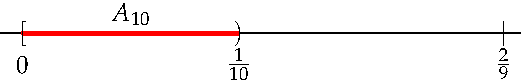
\includegraphics[width=0.5\textwidth]{setsii-06-intervalex}
\end{center}

\begin{proof}
We prove that $x\in\bigcap\limits_{n=1}^\infty A_n\iff x=0$.\\
Suppose that $x\in\bigcap\limits_{n=1}^\infty A_n$. Then $x\in\bigl[0\,,\,\frac 1n\bigr)$ for all $n$. Otherwise said,
\[\forall n\in\N,\text{ we have }0\le x<\frac 1n.\tag*{($\dag$)}\]
Certainly $x=0$ satisfies these inequalities.\\
Now suppose, for a contradiction, that $x>0$. Since $\lim\limits_{n\to\infty}\frac 1n=0$, we can certainly choose\footnote{Explicitly, you may choose choose $N=\lceil\frac 1x\rceil$, or anything larger. Here $\lceil x\rceil$ is the \emph{ceiling function:} the smallest integer greater than or equal to $x$.} $N$ large enough so that $\frac 1N\le x$. But this says that $x\not\in A_N$, which contradicts ($\dag$).\\
The intersection contains no positive elements, and we conclude that
\[\bigcap\limits_{n=1}^\infty A_n=\{0\}.\tag*{\qedhere}\]
\end{proof}

\noindent By modifying the sets $A_n$ to either include or exclude endpoints, we can obtain slightly different results. Consider each of the following in turn. How would the argument for computing each intersection differ from what we did above?
\begin{itemize}
  \item If $B_n=\Bigl(0\,,\,\frac 1n\Bigr)$, then $\bigcap\limits_{n=1}^\infty B_n=\emptyset$.
  \item If $C_n=\Bigl(0\,,\,\frac 1n\Bigr]$, then $\bigcap\limits_{n=1}^\infty C_n=\emptyset$.
  \item If $D_n=\Bigl[0\,,\,\frac 1n\Bigr]$, then $\bigcap\limits_{n=1}^\infty D_n=\{0\}$.
\end{itemize}
The moral of these examples is that you cannot naïvely apply limits to sequences of sets. Your intuition is often a good guide, but that doesn't mean you should trust it blindly!\\

Here are a few more examples.

 
\begin{examples}
	\item\label{ex:index2} Let $A_n=[n,n+1)\subseteq\R$, for each $n\in\Z$. For example,
\[A_3=[3,4),\quad\text{and}\quad A_{-17}=[-17,-16).\]
In this case the sets $A_n$ are pairwise disjoint, and we have
\[\bigcup\limits_{n\in\Z}A_n=\R,\quad\text{and}\quad\bigcap\limits_{n\in\Z}A_n=\emptyset.\]
To prove the former, note that $\forall x\in\R$ we have $x\in[n,n+1)$ where $n=\lfloor x\rfloor$ is the greatest integer which is less than or equal to $x$: i.e. $x\in A_{\lfloor x\rfloor}$.


	\item\vspace*{5pt} For each $n\in\N$, let $A_n=[-n,n]$. Each of the sets $A_n$ is a closed interval. E.g.,
	\[A_1=[-1,1],\qquad A_2=[-2,2],\qquad A_3=[-3,3].\]
	It should be clear that $n\le m\implies A_n\subseteq A_m$ so that we have a \emph{nested} sequence of sets:
	\[A_1\subseteq A_2\subseteq A_3\subseteq\cdots\]
	It follows immediately that the intersection is $\bigcap\limits_{n\in\N}A_n=A_1=[-1,1]$.\\
	With a little thinking you might hypothesize that the union is $\bigcup\limits_{n\in\N}A_n=\R$. To prove this, assume that $x\in\R$ is non-zero, and observe that
	\[-\lceil\nm x\rceil\le x\le\lceil\nm x\rceil\implies x\in A_{\lceil\nm x\rceil}\]
	Since $0\in A_1$, it follows that $\R\subseteq\bigcup\limits_{n\in\N}A_n$, whence these sets are equal.\\
	If the notation is causing difficulty, consider for example,
	\[-3.124\in A_{\lceil 3.124\rceil}=A_4.\]
	
	\item For each $n\in\N$, let $A_n=\{x\in\R:\nm{x^2-1}<\frac 1n\}$. Before computing the union and intersection of these sets, it is helpful to write each set as a pair of intervals. Note that
	\[\nm{x^2-1}<\frac 1n\iff -\frac 1n< x^2-1<\frac 1n\iff \sqrt{1-\frac 1n}< \nm x< \sqrt{1+\frac 1n}.\]
	Therefore
	\[A_n=\left(-\sqrt{1+\tfrac 1n},-\sqrt{1-\tfrac 1n}\right)\cup\left(\sqrt{1-\tfrac 1n},\sqrt{1+\tfrac 1n}\right).\]
	As the picture suggests, the sets $A_n$ are nested: $A_1\supseteq A_2\supseteq A_3\supseteq A_4\supseteq\cdots$.\\[5pt]
	\noindent\begin{minipage}{0.5\textwidth}
	Since $A_1$ is the largest of the nested sets, we see that
	\[\bigcup\limits_{n\in\N}A_n=A_1=(-\sqrt{2},0)\cup(0,\sqrt{2}).\]
	For the intersection, note that
	\begin{align*}
	\forall n\in\N,\ x\in A_n&\iff \forall n\in\N,\ \nm{x^2-1}<\frac 1n\\
	&\iff x^2-1=0.
	\end{align*}
	It follows that $\bigcap\limits_{n\in\N}A_n=\{1,-1\}$.
	\end{minipage}\hfill\begin{minipage}{0.38\textwidth}
	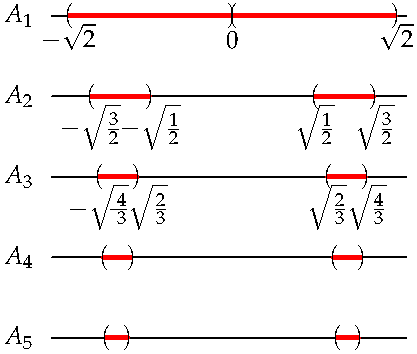
\includegraphics[width=\textwidth]{setsii-05-intervalex}
	\end{minipage}
\end{examples}


\subsubsection*{Indexed Unions: Don't Confuse Sets and Elements}

It is easy to confuse and important to distinguish between the sets
\[\{A_n:n\in I\}\qquad\text{and}\qquad\bigcup_{n\in I}A_n.\]
The first is a set whose \emph{elements} are themselves sets. The second is the collection of all elements in \emph{any} set $A_n$. Consider the following examples.


\begin{examples}
	\item For each $n\in\{1,2,3\}$, let $A_n$ be the plane $\{(x,y,z):x+ny+n^2z=1\}\subseteq\R^3$.\\[2pt]
	The indexed collection $\{A_1,A_2,A_3\}$ has \emph{three} elements: each of the planes $A_1,A_2,A_3$ is an element in its own right.\\
  The union $A_1\cup A_2\cup A_3$ is an \emph{infinite} set consisting of all the \emph{points} lying on any of the three planes.\\
  For the intersection, a little work with simultaneous equations should convince you that
  \[(x,y,z)\in\negthickspace\negthickspace\bigcap_{n\in\{1,2,3\}}\negthickspace\negthickspace A_n\iff
  \begin{cases}
  x+y+z=1\\
  x+2y+4z=1\\
  x+3y+9z=1
  \end{cases}\iff (x,y,z)=(1,0,0).\]
  Thus $\bigcap A_n=\{(1,0,0)\}$. The planes are drawn below.
  
  \item\label{ex:projline} Let $I=\R\cup\{\infty\}$. For each $m\in I$, let $A_m$ be the line\footnote{We include the vertical line $A_\infty$.} through the origin in $\R^2$ with gradient $m$.\\[2pt]
  Each element of $\{A_m:m\in I\}$ is a \emph{line}: there is one for each direction through the origin.\\
  The union $\bigcup A_m$ consists of all of the \emph{points} that lie on \emph{any} line through the origin. Since any point in the plane lies on some line through the origin, we see that $\bigcup A_m=\R^2$.\\
  It should be clear that all the lines intersect at the origin, and so $\bigcap A_m=\{(0,0)\}$.\\
  The collection of lines $\{A_m:m\in I\}$ is the famous \emph{projective space} $\mathbb P(\R^2)$; this is a very different set from $\R^2$!\\
  This example also shows that indexing sets don't have to be simple sets of integers. It is also possible to index the same set using $I=[0,\pi)$. If we define $B_\theta$ to be the line through the origin making an angle $\theta$ with the positive $x$-axis, we would then have $B_\theta=A_{\tan\theta}$.
\end{examples}

\begin{center}
\begin{minipage}[b]{0.45\textwidth}
\centering
\includemedia[width=0.8\textwidth, transparent=false, activate=onclick, add3Djscript=asylabels.js, add3Djscript=3Dspintool.js, 3Dmenu,
3Dcoo=-0.2646917402744293 -9.039887428283691 17.85630226135254,
3Dc2c=0.781423807144165 -0.5375411510467529 0.31690123677253723,
3Droo=261.5486749519297,
3Dlights=Headlamp]{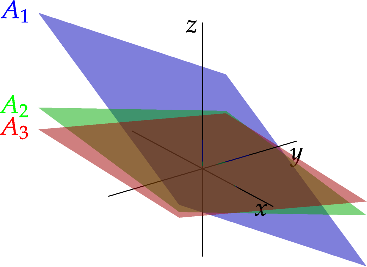
\includegraphics{setsii-01-planes+0_0}}{setsii-01-planes+0.prc}\\[15pt]
Example 1: Three elements, or an infinite number?
\end{minipage}\qquad\qquad
\begin{minipage}[b]{0.35\textwidth}
\centering
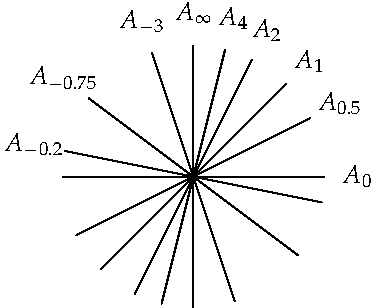
\includegraphics[width=\textwidth]{setsii-03-projective}\\
Example 2: Elements in $\mathbb P(\R^2)$
\end{minipage}
\end{center}


\subsubsection*{Finite Decimals}\label{ex:finitedec}

Here is another example where our intuition of `taking the limit' leads us astray. This time it is the union that behaves surprisingly.\\

\noindent For each $n\in\N$, let $A_n$ be the set of decimals of length $n$. That is
\[A_n=\bigl\{0.a_1a_2\ldots a_n:\text{where each $a_i\in\{0,1,\ldots,9\}$}\bigr\}.\]
For example $0.134\in A_3$. Since $0.134=0.1340$, we also have $0.134\in A_4$. Once again we have a nested sequence of sets
\[A_1\subseteq A_2\subseteq A_3\subseteq A_4\subseteq\cdots\]
The infinite intersection is therefore simply
\[\bigcap_{n\in\N}A_n=A_1=\{0,0.1,\ldots,0.9\}.\]
Now consider a finite union: if $m\in\N$, then
\[\bigcup_{n=1}^mA_n=A_m=\bigl\{x\in [0,1):x\text{ has a decimal representation of length $\le m$}\bigr\}.\]
At this point, we might be inclined to take the limit as $m\to\infty$ of the \emph{property} `length $m$ decimal.' If so, then it would seem that the infinite union should be the entire\footnote{We would include $1=0.9999\cdots$} interval $[0,1]$.\\
What is wrong with our reasoning? We have again abused the idea of limits: one cannot take the limit of a property! Instead we use the definition:
\begin{align*}
x\in\bigcup_{n\in\N}A_n&\iff\exists n\in\N\text{ such that }x\in A_n\\
&\iff\exists n\in\N \text{ such that $x$ is a decimal of length $n$.}
\end{align*}
It follows that
\[\bigcup_{n\in\N}A_n=\big\{x\in[0,1):x\text{ has a \emph{finite} decimal representation}\big\}\]
In particular, there are no irrational numbers in $\bigcup\limits_{n\in\N}A_n$:
\[\text{If $x\in A_n$, then $y=10^nx$ is an integer, whence $x=\frac y{10^n}\in\Q$.}\]
Many rational numbers are also excluded. For example $\frac 13=0.3333\cdots$ is not in any set $A_n$ and is therefore not in the union.


\subsubsection*{The Cantor Set}\label{ex:cantor}

We finish this section with a bit of fun. We can use infinite intersections to create self-similar sets, otherwise known as \emph{fractals.} The \emph{Cantor middle-third set} is a famous example.\\

\noindent Staring with the interval $C_0=[0,1]$, we construct a sequence of sets $C_n$ for each $n\in\N_0$ by repeatedly removing the middle third of each of the intervals contained in $C_n$.

\begin{minipage}{0.40\textwidth}
$C_0=[0,1]$,\\[4pt]
$C_1=[0,\frac 13]\cup [\frac 23,1]$,\\[4pt]
$C_2=[0,\frac 19]\cup [\frac 29,\frac 13]\cup [\frac 23,\frac 79]\cup [\frac 89,1]$, etc.
\end{minipage}
\begin{minipage}{0.55\textwidth}
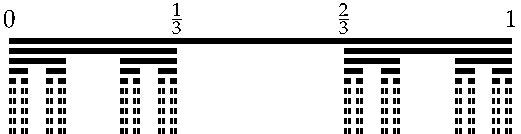
\includegraphics[width=\textwidth]{setsii-02-cantor}
\end{minipage}\\

\noindent The sequence is drawn up to $C_{9}$, with an animation below. To see the detail for the last few sets, try zooming in as far as you can.\vspace{-5pt}
\begin{center}
\animategraphics[width=\textwidth]{1}{setsii-07-cantor}{0}{9}
\end{center}\vspace{-8pt}

\begin{defn}
The \textbf{Cantor set} $\mathcal C$ is the infinite intersection $\mathcal C=\negthickspace\bigcap\limits_{n=0}^\infty\negthickspace C_n$.
\end{defn}

\noindent This set has several interesting properties.\\

\noindent{\bf Zero Measure} (length)\quad Intuitively, the \emph{length} of a set of real numbers is the sum of the lengths of all the intervals contained in the set. Since we start with the interval $[0,1]$ and remove a third of the set each time, it should be clear that
\[\operatorname{length}(C_0)=1,\qquad \operatorname{length}(C_1)=\frac 23,\qquad\operatorname{length}(C_2)=\left(\frac 23\right)^2,\quad\text{etc.}\]
Induction then gives us
\[\operatorname{length}(C_n)=\left(\frac 23\right)^n.\]
As $n\to\infty$ this goes to zero, so the Cantor set contains no intervals. This at least seems reasonable from the picture.\\

\noindent{\bf Infinite Cardinality}\quad The Cantor set $\mathcal{C}$ contains the endpoints of every interval removed at any stage of its construction. In particular, $\frac 1{3^n}\in\mathcal C$ for all $n\in\N_0$, and so $\mathcal C$ is an \emph{infinite} set. Indeed it is more than merely infinite, it is \emph{uncountably} so, as we shall see in Chapter \ref{sec:card}.\\

\noindent{\bf Self-similarity}\quad If $\frac 13\mathcal C$ means `take all the elements of $\mathcal C$ and divide them by three,' and $\frac 13\mathcal C+\frac 23$ means `take all the elements of $\frac 13\mathcal C$ and add $\frac 23$,' then
\[\mathcal C=\frac{\mathcal C}{3}\cup\left(\frac{\mathcal C}{3}+\frac 23\right).\tag*{($\ast$)}\]
Otherwise said, $\mathcal C$ is made up of two shrunken copies of itself, a classic property of fractals. If you were to zoom into the Cantor set far enough that you couldn't see the whole set, you would not know what the scale was. In the following animation we are repeatedly zooming in on the second (of four) groups of points.
\begin{center} 
\animategraphics[width=0.6\textwidth,loop]{6}{setsii-08-cantor}{0}{22}
\end{center}

\subsubsection*{Optional: Analyzing the Cantor Set}

To get further with the Cantor set, it is necessary to explicitly describe the elements of the set. This can be accomplished using the \emph{ternary representation.}\label{page:cantor} It can be shown that every number $x\in[0,1]$ may be written in the form\footnote{Analogous to a decimal representation $x=\sum\limits_{n=1}^\infty 10^{-n}a_n=\frac{a_1}{10}+\frac{a_2}{10^2}+\frac{a_3}{10^3}+\cdots$ where $a_n\in\{0,1,2,\ldots,9\}$.}
  \[x=\sum\limits_{n=1}^\infty 3^{-n}a_n=\frac{a_1}{3}+\frac{a_2}{3^2}+\frac{a_3}{3^3}+\cdots\]
  where each $a_n\in\{0,1,2\}$. We write $x=[0.a_1a_2a_3\cdots]_3$. For example:
\[[0.12]_3=\frac 13+\frac 2{3^2}=\frac 59,\qquad \frac{64}{243}=\frac 2{3^2}+\frac 1{3^3}+\frac 1{3^5}=[0.02101]_3,\qquad 1=[0.22222\cdots]_3.\]
For this last, use the formula for the sum of a geometric series to calculate $\sum\limits_{n=1}^\infty 2\left(\frac 13\right)^n=2\cdot\frac{1/3}{1-1/3}=1$.\\
To convince yourself of the existence of a ternary representation, note that if $0\le x<1$ it follows that $x<3$ and so, we can take
\[a_1=\lfloor 3x\rfloor\in\{0,1,2\}\]
Now repeat, with $a_2=\lfloor x-\frac{a_1}3\rfloor$, etc.
  It can also be shown that the only possibility whereby $x$ can have two ternary expansions is if one of them terminates. The other will eventually become a sequence of repeating 2's. For example:\footnote{This is ticklish to prove, as is the corresponding result for decimals: compare with $1=0.99999999\cdots$}
  \[[0.0222222\cdots]_3=[0.1]_3=\frac 13\quad \text{and}\quad [0.10122222\cdots]_3=[0.102]_3=\frac 13+\frac 2{27}=\frac{11}{27}.\]
  We can now describe precisely the elements of each of the sets $C_n$ and consequently the Cantor set.

\begin{thm}
$C_n$ is the set of all numbers $x\in[0,1]$ with a ternary expansion whose first $n$ digits are only 0 or 2. It follows that $\mathcal C$ is the set of $x\in[0,1]$ with a ternary expansion containing only 0 and 2.
\end{thm}

\noindent The Theorem tells us that the Cantor set contains \emph{a lot} of elements. For example:
\[[0.020202020\cdots]_3=2\sum_{n=1}^\infty 3^{-2n}=\frac{2/9}{1-1/9}=\frac 14\]
is an element of the Cantor set! What is strange is that $\frac 14$ is not the endpoint of any of the open intervals deleted during the construction of $\mathcal C$, and yet we've already established that $\mathcal C$ contains no intervals! Cantor introduced his set precisely because it was so challenging to the traditional concept of size: $\mathcal C$ seems to simultaneously have very few elements and enormously many.

\begin{proof}
We prove by induction.\\[2pt]
(\emph{Base Case})\quad The proposition is clearly true for $C_0=[0,1]$, as there is nothing to check.\\[2pt]
(\emph{Induction Step})\quad Assume that the proposition is true for some fixed $n\in\N_0$. Analogously to ($\ast$) above, observe that $C_{n+1}$ is built from two shrunken copies of $C_n$:
\[C_{n+1}=\frac 13C_n\cup\left(\frac 13C_n+\frac 23\right).\]
Now consider what division by 3 and addition of $\frac 23$ does to a ternary representation.
\begin{itemize}
  \item Since $\frac 13\sum_{n=1}^\infty 3^{-n}a_n=\sum_{n=1}^\infty 3^{-n-1}a_1$, we see that multiplication by $\frac 13$ shifts a ternary representation one position to the right.\footnote{Compare to multiplication of a decimal by $\frac 1{10}$.}
	\[\frac 13[0.a_1a_2a_3\ldots]_3=[0.0a_1a_2a_3\ldots]_3\]
	\item Since $\frac 23=[0.2]_3$ we see that
	\[\frac 23+\frac 13[0.a_1a_2a_3\ldots]_3=[0.2a_1a_2a_3\ldots]_3\]
\end{itemize}
By the induction hypothesis, $C_n$ contains only 0's and 2's in its first $n$ entries. By moving ternary representations one step to the right and inserting 0 or 2 in the first position, we conclude that $C_{n+1}$ contains only 0's and 2's in its first $n+1$ entries.\\[2pt]
By induction the proposition is true for all $n\in\N_0$.
\end{proof}

\noindent Other fractal sets based on $\mathcal C$ include the Cantor dust $\mathcal C\times\mathcal C$, the \href{http://en.wikipedia.org/wiki/Sierpinski_carpet}{Sierpi\'nski carpet} and \href{http://en.wikipedia.org/wiki/Sierpinski_triangle}{gasket}, and the \href{http://en.wikipedia.org/wiki/Koch_snowflake}{von Koch snowflake.}



% \paragraph{Self-test Questions}

% 	\begin{enumerate}
%     \item If $\{A_n:n\in I\}$ is a collection of sets then
%     \begin{enumerate}
%       \item $x\in \bigcap_{n\in I}A_n\iff$ \underline{\phantom{$\exists n\in I:x\in A_n$,\qquad}}
%       \item $x\in \bigcup_{n\in I}A_n\iff$ \underline{\phantom{$\forall n\in I:x\in A_n$,\qquad}}
%   \end{enumerate}
%     \item For any real number $x$, the \emph{ceiling} function applied to $x$ is the value $\lceil x\rceil$, which is defined to be \underline{\phantom{the least integer greater than or equal to $x$\qquad}}
%     \item What does it mean for a collection of sets $\{A_n:n\in\N\}$ to be \emph{nested?}
%     \item True or false:
%     \begin{gather*}
%     B\subseteq \bigcup_{n\in I}A_n\iff \forall n\in I,\ B\subseteq A_n
%     \end{gather*}
%   \end{enumerate}

\subsection*{Reading Quiz}

\begin{enumerate}
\item Let $I$ be a set and $\{A_n : n \in I\}$ a family of sets indexed by $I$. Then the definition of $\bigcup_{n \in I} A_n$ uses the \rule{2.5cm}{0.15mm} quantifier and the definition of $\bigcap_{n \in I} A_n$ uses the \rule{2.5cm}{0.15mm} quantifier.
\begin{enumerate}
    \item existential; existential
    \item existential; universal
    \item universal; existential
    \item universal; universal
\end{enumerate}

\item Let $I$ be a set and $\{A_n : n \in I\}$ a collection of sets indexed by $I$ which is nested. What can you conclude? Select all that apply.
\begin{enumerate}
    \item $\bigcap_{n \in I} A_n \neq \emptyset$.
    \item $\bigcup_{n \in I} A_n = A_1$.
    \item The collection of sets is pairwise disjoint.
    \item Each $A_n$ must be an interval.
\end{enumerate}

\item True or False:
\[
    B\subseteq \bigcup_{n\in I}A_n\iff \forall n\in I,\ B\subseteq A_n
\]
\end{enumerate}

\subsection*{Practice Problems}

\begin{enumerate}\renewcommand{\labelenumi}{\thesubsection.\theenumi}
\item (From previous exercises) For each non-negative real number $r\ge 0$ let 
  \[A_r=\big\{(x,y)\in\R^2:x^2+y^2=r^2\big\}\]
		\begin{enumerate}
  		\item Describe each of the sets $A_r$ geometrically.
  		\item Prove that $\bigcup_{r\in\R^+_0}A_r=\R^2$.
		\end{enumerate}
		
		\href{https://youtu.be/WuSucjuxjbU}{Video Solution}
		
\item Let $I$ be a set, $\{A_n : n \in I\}$ a family of sets indexed by $I$ and $B$ a set. Prove:
\begin{enumerate}
    \item \[ \left(\bigcup_{n \in I} A_n \right) \cap B = \bigcup_{n \in I} (A_n \cap B) \]
    \item \[ \left(\bigcap_{n \in I} A_n \right) \cup B = \bigcap_{n \in I} (A_n \cup B) \]
\end{enumerate}

\href{https://youtu.be/CtIg2lrsyAs}{Video Solution}

\end{enumerate}

\subsection*{Exercises}

\begin{enumerate}\renewcommand{\labelenumi}{\thesubsection.\theenumi}
  	\item For each integer $n$, consider the set $B_n=\{n\}\times\R$.
	\begin{enumerate}
		\item Draw a picture of $\bigcup\limits_{n=2}^4B_n$ (in the Cartesian plane).\\
		\emph{Hint}:  $\bigcup \limits_{n=2}^{4} B_n= B_2 \cup B_3 \cup B_4.$
		\item Draw a picture of the set $C=[1,5]\times\{-2,2\}.$
		\emph{Careful!} $[1,5]$ is an interval, while $\{-2,2\}$ is a set containing two points.
		\item Compute $\left(\bigcup\limits_{n=2}^4B_n\right)\cap C$.
		\item Compute $\bigcup\limits_{n=2}^4\left(B_n\cap C\right)$.
		\item Compare $\left(\bigcup\limits_{n=2}^4B_n\right)\cap C$ and $\bigcup\limits_{n=2}^4\left(B_n\cap C\right)$. What do you notice?
	\end{enumerate}

  \item \begin{enumerate} \item Determine $\bigcup\limits_{r\in \{1,3,4\}}S_r$ and $\bigcap\limits_{r\in \{1,3,4\}}S_r$, where $S_r$ is the interval $[r-1,r+3]$.
  \item Determine $\bigcup\limits_{i\in \N} \{i\}$ and $\bigcap\limits_{i\in \N} \{i\}$.

\item Determine $\bigcup\limits_{X\in \cP{(\Z)}} X$ and $\bigcap\limits_{X\in \cP{(\Z)}} X$ .
\end{enumerate}

  \item Give an example of four different subsets $A,B,C$ and $D$ of $\{1,2,3,4\}$ such that all intersections of two subsets are different.

  \item Find both the union and intersection of the following indexed collections of intervals. (Hint: Start by drawing a few sets in each collection.)
   \begin{enumerate}
     \item $\{A_n\}_{n\in\N} = \big\{[0,2+n] \colon  n \in \N\}$
     \item $\{A_n\}_{n\in\N} = \big\{[1,2+1),\,[1,2+\frac 12),\,[1,2+\frac 13),\,\ldots\big\}$
     \item $\{A_n\}_{n\in\N} =  \big\{(\frac{-2n+1}{n},2n)  \colon  n \in \N\} $
     \item $\{A_n\}_{n\in\N} = \big\{(\frac 14,1),\,(\frac 18,\frac 12),\,(\frac 1{16},\frac 14),\,(\frac 1{32},\frac 18), \,(\frac 1{64},\frac 1{16}),\,\ldots\big\}$
   \end{enumerate}
  
  \item For each non-negative real number $r\ge 0$ let 
  \[A_r=\big\{(x,y)\in\R^2:x^2+y^2=r^2\big\}\]
		\begin{enumerate}
  		\item Describe each of the sets $A_r$ geometrically.
  		\item Prove that $\bigcup_{r\in\R^+_0}A_r=\R^2$.
		\end{enumerate}

  \item For each real number $x$, let $A_x=\{3,-2\}\cup\{y\in\R:y>x\}$. Find $\bigcup\limits_{x\in\R}A_x$ and $\bigcap\limits_{x\in\R}A_x$.
  
  \item Use Definition \ref{defn:indexed} to prove the following results about nested sets.
		\begin{enumerate}
  		\item $A_1\supseteq A_2\supseteq A_3\supseteq\cdots\implies \bigcup\limits_{n\in\N}A_n=A_1$.
  		\item $A_1\subseteq A_2\subseteq A_3\subseteq\cdots\implies \bigcap\limits_{n\in\N}A_n=A_1$.
		\end{enumerate}

  \item Let $C_0(\R)$ denote the set of continuous functions $f:\R\to\R$ which satisfy $f(0)=0$.\\
  Let $A_f=\{x\in[0,1]:f(x)=0\}$ (so, for example, if $f:\R\to\R,\,x \mapsto x(2x-1)$, then $A_f=\{0,\frac 12\}$).
    \emph{Prove} that
  \[\bigcup\limits_{f\in C_0(\R)}\negthickspace\negthickspace A_f=[0,1]\qquad\text{and}\qquad\bigcap\limits_{f\in C_0(\R)}\negthickspace\negthickspace A_f=\{0\}.\]
		
	\item Let $A_n$ be the set of decimals of length $n$, as described on page \pageref{ex:finitedec}.
		\begin{enumerate}
	  	\item Prove directly that the cardinality of $A_n$ is $10^n$.
	  	\item Prove by induction that $\nm{A_n}=10^n$.
	  	\item Prove that $\bigcup\limits_{n=1}^\infty A_n\subseteq\Q$.
			\item Prove by contradiction that $\frac 13\not\in\bigcup\limits_{n=1}^\infty A_n$.
		\end{enumerate}

  \item Suppose that the following are true:
  \begin{itemize}
    \item $\forall n\in\N$, $A_n\neq\emptyset$.
    \item $m\ge n\Longrightarrow A_m\subseteq A_n$.
  \end{itemize}
  Prove or disprove the following conjectures:\\
	\begin{minipage}{0.4\textwidth}
  \begin{enumerate}
    \item $\bigcup\limits_{n=1}^{293}A_n\neq\emptyset$
    \item $\bigcap\limits_{n=1}^{293}A_n\neq\emptyset$
	\end{enumerate}
	\end{minipage}
	\begin{minipage}{0.4\textwidth}
  \begin{enumerate}\setcounter{enumii}{2}
    \item $\bigcup\limits_{n\in\N}^{\phantom{293}}A_n\neq\emptyset$
		\item $\bigcap\limits_{n\in\N}^{\phantom{293}}A_n\neq\emptyset$
	\end{enumerate}
	\end{minipage}
	
	\item Suppose we are working in a universal set $\cU$ (so every set is considered a subset of $\cU$). Give an explanation for why it makes sense to define $\bigcap_{n \in I} A_n = \cU$ when $I = \emptyset$.

\item Let $\{A_n : n \in I\}$ and $\{B_n : n \in I\}$ be indexed families of sets. Give explicit examples for which the following hold:
\begin{enumerate}
    \item \[\left(\bigcup_{n \in I} A_n \right) \cap \left(\bigcup_{n \in I} B_n \right) \neq \bigcup_{n \in I} (A_n \cap B_n)\]
    \item \[\left(\bigcap_{n \in I} A_n \right) \cup \left(\bigcap_{n \in I} B_n \right) \neq \bigcap_{n \in I} (A_n \cup B_n)\]
\end{enumerate}

\item (De Morgan's laws) Let $\{A_n : n \in I\}$ be an indexed family of sets and $B$ a set. Prove
\begin{enumerate}
    \item \[B \setminus \left(\bigcup_{n \in I} A_n \right) = \bigcap_{n \in I} (B \setminus A_n)\]
    \item \[B \setminus \left(\bigcap_{n \in I} A_n \right) = \bigcup_{n \in I} (B \setminus A_n)\]
\end{enumerate}

\item Let $\{A_n : n \in I\}$ be an indexed family of sets and $B$ a set. Prove
\begin{enumerate}
    \item \[\left(\bigcup_{n \in I} A_n \right) \setminus B = \bigcup_{n \in I} (A_n \setminus B)\]
    \item \[\left(\bigcap_{n \in I} A_n \right) \setminus B = \bigcap_{n \in I} (A_n \setminus B)\]
\end{enumerate}\

\item We can take the Cartesian product of arbitrarily many sets. Let $\{A_n : n \in I\}$ be a family of sets. Define
\[
\prod_{n \in I} A_n = \left\{f : I \to \bigcup_{n \in I} A_n \bigm| f(n) \in A_n\right\}.
\]
\begin{enumerate}
    \item If $I = \N$ and $A_n = \R$ for each $n \in \N$, can you give a more intuitive description of the elements of $\prod_{n \in \N} A_n$?
    \item Suppose we have two families $\{A_n : n \in I\}$ and $\{B_n : n \in I\}$. Prove
    \[
        \left(\prod_{n \in I} A_n \right) \cap \left(\prod_{n \in I} B_n \right) = \prod_{n \in I} (A_n \cap B_n)
    \]
\end{enumerate}

	\item (Hard) Let $A_n=\{\frac mn\in\Q:0<m<n, m\in \N\}$, for each $n\in\N$.
	\begin{enumerate}
		\item Write down $A_1,A_2,A_3,A_4$ explicitly.
		\item Prove that $A_m\subseteq A_{pm}$ for any $p\in\N$.
		\item Argue that $\bigcup\limits_{n\in\N}A_n=\Q\cap (0,1)$.
		\item Argue that further $\bigcup\limits_{n\in\N}A_{2n}=\Q\cap (0,1)$.
		\item Extend your proof to show that, for any fixed $p\in\N$, $\bigcup\limits_{n\in\N}A_{pn}=\Q\cap (0,1)$.
	\end{enumerate}
	
	\item In this question we construct a fractal shape, similar to the von Koch curve. Let $F_0=[0,1]$ be a straight line of length 1. Delete the segment between $\frac 12$ and $\frac 34$ to obtain the set
    \[F_1=[0,\tfrac 12]\cup[\tfrac 34,1]\]
    Now repeat: delete the third quarter of each of the two line segments in $F_1$ to obtain
    \[F_2=[0,\tfrac 14]\cup[\tfrac 38,\tfrac 12]\cup[\tfrac 34,\tfrac 78]\cup[\tfrac{15}{16},1]\]
    Suppose we repeat this process to create an infinite sequence of sets $F_0,F_1,F_2,F_3,F_4,\ldots$
  \begin{enumerate}
    \item Prove that the total length of all of the line segments making up the set $F_n$ is $\left(\frac 34\right)^n$.
    \item Prove by contradiction that the intersection $\bigcap\limits_{n=1}^\infty F_n$ does not contain any intervals of positive length.
    \item Now suppose that instead of simply deleting the third quarter of each line segment at each step, we replace it with the other three sides of a square. The first three steps in this process are shown below.
    \begin{center}
    \begin{tabular}{ccc}
    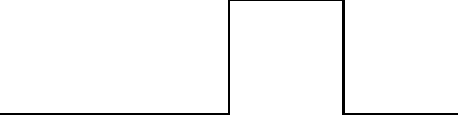
\includegraphics[width=0.27\textwidth]{fractal1}
    &
    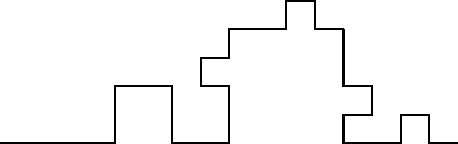
\includegraphics[width=0.27\textwidth]{fractal2}
    &
    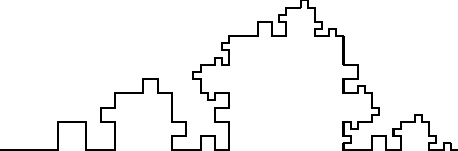
\includegraphics[width=0.27\textwidth]{fractal3}
   	\\
   	Step 1&Step 2&Step 3
    \end{tabular}
    \end{center}
    After each step, we are left with a curve. After step 1 the curve has length $\ell_1=\frac 32$. After step 2 the length is $\ell_2=\frac 94$. What is the \emph{length} $\ell_n$ of the curve after $n$ steps? Prove your assertion.
    \item Below is the result of repeating the steps in part 3 infinitely many times. What is the `length' of the resulting fractal curve?
    \begin{center}
    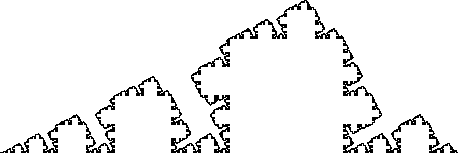
\includegraphics[width=0.75\textwidth]{fractal}
    \end{center}
    \item Repeat parts (c) and (d) for the \emph{area} under the curve at each step. Prove that the area between the fractal curve and the $x$-axis is $\frac 18$.
	\end{enumerate}
	
	\item Let $X$ be a set. A collection of sets $\tau \subseteq \cP(X)$ is called a \emph{topology} if the following conditions are satisfied:
\begin{enumerate}[label=(\arabic*)]
    \item $\emptyset \in \tau$ and $X \in \tau$;
    \item $\tau$ is closed under arbitrary union. That is, if $\{U_n : n \in I\} \subseteq \tau$ for any index set $I$, then $\bigcup_{n \in I} U_n \in \tau$;
    \item $\tau$ is closed under finite intersection. That is, if $U_1,\ldots,U_n \in \tau$ for any $n \in \N$, then $U_1 \cap \cdots \cap U_n \in \tau$.
\end{enumerate}
Elements of $\tau$ are called \emph{open sets}.
\begin{enumerate}
    \item Let $X = \{a,b,c,d\}$. Let $\tau_1 = \{\emptyset, X\}$, $\tau_2 = \cP(X)$, $\tau_3 = \{\emptyset, \{d\}, \{a,b\}, \{b,c\}, \{a,b,c\}, X\}$, and $\tau_4 = \{\emptyset, \{b\}, \{a,b\}, \{b,c\}, \{a,b,c\}, X\}$. Show $\tau_1,\tau_2$ and $\tau_4$ are topologies while $\tau_3$ is not.
    
    \item Let $X$ be an infinite set and define $\tau = \{A \in \cP(X) : X \setminus A \text{ is finite}\} \cup \{\emptyset\}$. Show $\tau$ is a topology.
    \item The \emph{standard topology} $\tau$ on $\R$ can be defined by declaring that a set $U \subseteq \R$ is open (i.e. an element of $\tau$) if and only if for every $x \in U$, there is an open interval $(a,b)$ such that $x \in (a,b)$ and $(a,b) \subseteq U$. Show this defines a topology on $\R$.
\end{enumerate}

\item Let $X$ be a set and $\tau$ a topology on $X$. A set $C \subseteq X$ is called \emph{closed} if its complement is open, i.e., if $X \setminus C \in \tau$. 
\begin{enumerate}
    \item Show the following properties of closed sets:
    \begin{enumerate}[label=(\roman*)]
        \item $\emptyset$ and $X$ are both closed.
        \item If $\{A_n : n \in I\}$ is an arbitrary collection of closed sets, then $\bigcap_{n \in I} A_n$ is closed.
        \item If $A_1,\ldots,A_n$ are closed sets, then $A_1 \cup \cdots \cup A_n$ is closed.
    \end{enumerate}
    \item In the standard topology on $\R$, show that a closed interval $[a,b]$ is a closed set but that a half-open interval $[a,b)$ is neither open nor closed.
\end{enumerate}
\end{enumerate}